\documentclass[11pt,a4paper,ngerman]{article}
\usepackage[bottom=2.5cm,top=2.5cm]{geometry} 
\usepackage{babel}
\usepackage[utf8]{inputenc} 
\usepackage[T1]{fontenc} 
\usepackage{ae} 
\usepackage{amssymb} 
\usepackage{amsmath}
\usepackage{amsthm} 
\usepackage{graphicx}
\usepackage{fancyhdr}
\usepackage{fancyref}
\usepackage{listings}
\usepackage{xcolor}
\usepackage{paralist}

\usepackage[pdftex, bookmarks=false, pdfstartview={FitH}, linkbordercolor=white]{hyperref}
\usepackage{fancyhdr}
\pagestyle{fancy}
\fancyhead[C]{Advanced Functional Programming}
\fancyhead[L]{Exercise sheet 2}
\fancyhead[R]{SoSe 2013}
\fancyfoot{}
\fancyfoot[L]{}
\fancyfoot[C]{\thepage \hspace{1px} of \pageref{LastPage}}
\renewcommand{\footrulewidth}{0.5pt}
\renewcommand{\headrulewidth}{0.5pt}
\setlength{\parindent}{0pt} 
\setlength{\headheight}{0pt}

\date{}
\title{Exercise sheet 2}
\author{Max Wisniewski, Alexander Steen}


%%
%% Enviroments for proofs and lemmas
%%
\newtheorem{lemma}{\bfseries lemma}
\newtheorem{claim}{\bfseries claim}
\newtheorem{theorem}{\bfseries Theorem}

\lstloadlanguages{Haskell}
\lstset{
  language=Haskell,
  basicstyle=\ttfamily,
  flexiblecolumns=false,
  basewidth={0.5em,0.45em},
  literate={+}{{$+$}}1 {/}{{$/$}}1 {*}{{$*$}}1 {=}{{$=$}}1
           {>}{{$>$}}1 {<}{{$<$}}1 {\\}{{$\lambda$}}1
           {\\\\}{{\char`\\\char`\\}}1
           {->}{{$\rightarrow$}}2 {>=}{{$\geq$}}2 {<-}{{$\leftarrow$}}2
           {<=}{{$\leq$}}2 {=>}{{$\Rightarrow$}}2 
           {\ .}{{$\circ$}}2 {\ .\ }{{$\circ$}}2
           {>>}{{>>}}2 {>>=}{{>>=}}2
           {|}{{$\mid$}}1               
}

\lstnewenvironment{code}
    {\lstset{basicstyle=\footnotesize\ttfamily}%
      \csname lst@SetFirstLabel\endcsname}
    {\csname lst@SaveFirstLabel\endcsname}
\long\def\ignore#1{}

\begin{document}

\renewcommand{\figurename}{Figure}
\maketitle
\thispagestyle{fancy}

\documentclass[11pt,a4paper,ngerman]{article}
\usepackage[bottom=2.5cm,top=2.5cm]{geometry}
\usepackage[ngerman]{babel}
\usepackage[utf8]{inputenc}
\usepackage[T1]{fontenc}
\usepackage{ae}
\usepackage{amssymb}
\usepackage{amsmath}
\usepackage{amsthm}
\usepackage{graphicx}
\usepackage{fancyhdr}
\usepackage{fancyref}
\usepackage{listings}
\usepackage{xcolor}
\usepackage{stmaryrd}
\usepackage{paralist}
\usepackage{tikz}
\usepackage{amsthm}

\usetikzlibrary{arrows,automata}

\newtheorem{propo}{Satz}
\newtheorem{lemmas}[propo]{Lemma}

\usepackage[pdftex, bookmarks=false, pdfstartview={FitH}, linkbordercolor=white]{hyperref}
\usepackage{fancyhdr}
\pagestyle{fancy}
\fancyhead[C]{ADS}
\fancyhead[L]{Übung 3}
\fancyhead[R]{SoSe 2014}
\fancyfoot{}
\fancyfoot[L]{}
\fancyfoot[C]{\thepage \hspace{1px} von \pageref{LastPage}}
\renewcommand{\footrulewidth}{0.5pt}
\renewcommand{\headrulewidth}{0.5pt}
\newcommand{\set}[1]{ \{ #1 \}}
\setlength{\parindent}{0pt}
\setlength{\headheight}{0pt}

\newcommand{\N}{\mathbb{N}}
\newcommand{\Q}{\mathbb{Q}}
\newcommand{\R}{\mathbb{R}}
\newcommand{\bigO}{\mathcal{O}}
\newcommand{\Rarr}{\Rightarrow}
\newcommand{\rarr}{\rightarrow}
\newcommand{\Pot}{\mathcal{P}}
\newcommand{\abs}[1]{\left |#1\right|}
\newcommand{\solved}{$\mbox{}$ \hfill $\square$}
\newcommand{\Epsilon}{\mathcal{E}}

\newcommand{\erw}[1]{\text{\bfseries E} \left[ #1 \right]}
\newcommand{\prob}[1]{\text{Pr}\left[ #1 \right]}

\date{}
\title{Übung 3}
\author{Max Wisniewski, Melanie Skodzik}


%%
%% Enviroments for proofs and lemmas
%%
\newtheorem{prop}{\bfseries Behauptung}
\newtheorem{lemma}{\bfseries Lemma}

\begin{document}

\lstset{language=Pascal, basicstyle=\ttfamily\fontsize{10pt}{10pt}\selectfont\upshape, commentstyle=\rmfamily\slshape, keywordstyle=\rmfamily\bfseries, breaklines=true, frame=single, xleftmargin=3mm, xrightmargin=3mm, tabsize=2, mathescape=true}

\renewcommand{\figurename}{Grafik}

\maketitle
\thispagestyle{fancy}


\subsection*{Aufgabe 1}

\subsubsection*{(a)}
Seien $T_1$ und $T_2$ zwei binäre Suchbäume mit Schlüsselmenge $\{1, \ldots, n\}$. Zeigen Sie, dass sich $T_1$ mit $O(n)$ Rotationen in $T_2$ konvertieren lässt. Bestimmen Sie die Anzahl der Rotationen für Ihre Strategie im schlimmsten Fall exakt.

Versuchen Sie, so effizient wie möglich zu sein.\\

\noindent\textbf{Beweis:}\\

In unserem Algorithmus werden wir nur in der Wurzel des gerade betrachteten Baumes rotieren. 

Im folgenden bezeichnen $t_1,t_2$ die Wurzeln der Bäume $T_1$ und $T_2$, sowie $l_1,l_2, r_1, r_2$ die unmittelbaren linken und rechten Kinder.\\

Sei o.B.d.A. $t_1 \leq t_2$. Nun haben wir 5 Mögliche Fälle (im anderen Fall
sind die ersten beiden Symmetrisch zu einander) zu betrachten:
\begin{enumerate}[1.]
   \item $t_1 < t_2$ und $t_1 \geq r_2$:\\
      Falls $l_1 < t_2$, müssen wir $l_1$ und seinen linken Teilbaum
      links der Wurzel lassen, da sie auch im resultierenden Baum dort stehen.\\
      Wir machen erst eine Rechtsrotation um $l_1$ und dann eine Rechtsrotation
      um die Wurzel.\\
      Im anderen Fall nur eine einfache Rechtsrotation um $t_1$.\\
      Beobachtung: Komplett $r_2$ stehen schon im Richtigen Teilbaum und müssen
      nicht mehr über diesen Knoten (egal was später drin steht) verschoben werden.
      Im ersten Fall ist $l_1$ und der linke Unterbaum schon an der richtigen 
      Stelle. Beim zweiten Fall wissen wir, dass der rechte Unterbaum von $l_1$
      nun auf jeden Fall auf der richtigen Seite von $t_1$ steht.
   \item $t_1 < t_2$ und $t_1 < r_2$:\\
      Wie im letzten Fall schauen wir, ob $l_1 < t_2$ ist und führen zunächst
      eine Linksrotation um $l_1$ aus, falls $l_1$ kleiner ist. Sonst in jedem Fall ein      Rechtsrotation.\\
      Nun führen wir noch im rechten Teilbaum wo nun $t_1$ steht 
      eine eine Linksrotation aus.\\
      Beobachtung: Sowohl $t_1$ als auch die Knoten der inneren beiden Unterbäume 
      müssen nicht mehr über die Position von $r$ Verschoben werden.
   \item $t_1 = t_2$:\\
      Fahre Rekursiv mit mit den beiden Unterbäumen fort.\\
      Beobachtung:\\
      Aufgrund der Sortierung sollte nie ein Knoten über die Wurzel wandern müssen.
\end{enumerate}

Wir definieren nun zunächst für einen Knoten $x \in \{1, \ldots, n \}$ den Wert 
$\Delta_T(x)$ als die Länge des Weges im vollständigen Baum um von seiner Position
in $T$ zu seiner Position in $T_2$ zu kommen.\\


Wir sehen zunächst, dass $\Delta_{T_1}(x) \leq 2(n-1)$ für alle $x \in \{1, \ldots, n \}$, da die maximale Tiefe eines Baumes mit $n$ Knoten $n-1$ ist.\\

Wir definieren die Unordnung $\mathcal{U}(T) = \underset{x \in T}{\max} \Delta_T(x)$.\\

\begin{lemmas} \label{ads:ueb3:aufr} (Aufräumlemma)\\
   Die maximale Pfadlänge zur Ordnung wird in jedem Schritt um mindestens eins kleiner.   D.h. für $T$ BSB über $\{1, \ldots, n\}$ und $T'$ BSB von $T$ nach Ausführung eines
   Schrittes des Algorithmus gilt
   $$
      \mathcal{U}(T') \leq \mathcal{U}(T) - 1.
   $$
\end{lemmas} 


\noindent\textbf{Beweis \ref{ads:ueb3:aufr}.}\\

tbd

\subsubsection*{(b)}

Sei $n=5$. Betrachte Sie die Anfragefolge $\sigma = 2,1,5,1,2,4,4,2,3,5$. Bestimmen Sie $I(\sigma)$. Geben Sie eine möglichst gute Bearbeitungsstrategie für $\sigma$ an. Berechnen Sie die Kosten für Ihren Algorithmus und vergleichen Sie sie mit $I(\sigma)$.\\

\noindent\textbf{Lösung:}\\

Im vollständigen Baum befinden sich $4,2,1$ auf dem linken Pfad. Es wird also das erste mal bei Anfrage $3$ auf die 5 ein rechter Pfad Liebling, der danach sofort wieder auf links gesetzt wird. Nun bleiben wir bis zu den letzten beiden Anfragen auf links. Bei den letzten beiden gehen wir genau 2 mal nach Rechts, wobei wir vorher auf links waren.\\

Demnach ist $I(\sigma) = 3$.\\

Bei der optimalen Strategie für $\sigma$ sind wir uns unsicher, mit welchem Baum wir starten, deswegen geben wir uns schon einen möglichst guten Baum vor.

\begin{center}
   1.
   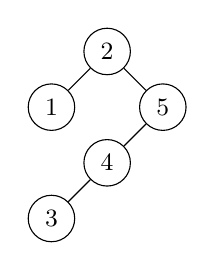
\begin{tikzpicture}[font=\small, minimum size=0.5cm]
      \node[circle, draw=black,name=a] {$2$};
      \node[circle, draw=black, name=b, below left of=a] {$1$};
      \node[circle, draw=black, name=c, below right of =a] {$5$};
      \node[circle, draw=black, name=d, below left of = c] {$4$};
      \node[circle, draw=black, name=e, below left of =d] {$3$};

      \path[-]
         (a) edge (b)
         (a) edge (c)
         (c) edge (d)
         (d) edge (e);
   \end{tikzpicture}
   2.
    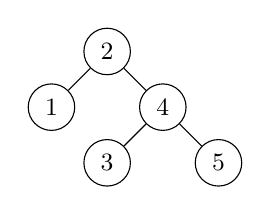
\begin{tikzpicture}[font=\small, minimum size=0.5cm]
      \node[circle, draw=black,name=a] {$2$};
      \node[circle, draw=black, name=b, below left of=a] {$1$};
      \node[circle, draw=black, name=c, below right of =a] {$4$};
      \node[circle, draw=black, name=d, below left of = c] {$3$};
      \node[circle, draw=black, name=e, below right of =c] {$5$};

      \path[-]
         (a) edge (b)
         (a) edge (c)
         (c) edge (d)
         (c) edge (e);
   \end{tikzpicture}
   3.
  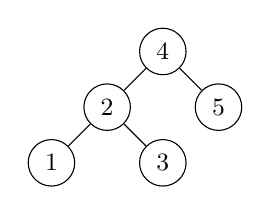
\begin{tikzpicture}[font=\small, minimum size=0.5cm]
      \node[circle, draw=black,name=a] {$4$};
      \node[circle, draw=black, name=b, below left of=a] {$2$};
      \node[circle, draw=black, name=c, below left of =b] {$1$};
      \node[circle, draw=black, name=d, below right of = b] {$3$};
      \node[circle, draw=black, name=e, below right of =a] {$5$};

      \path[-]
         (a) edge (b)
         (b) edge (c)
         (b) edge (d)
         (a) edge (e);
   \end{tikzpicture}
   4.
   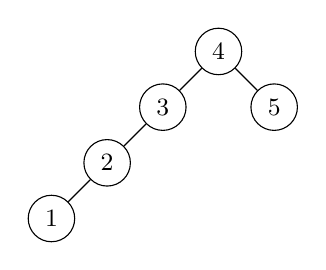
\begin{tikzpicture}[font=\small, minimum size=0.5cm]
      \node[circle, draw=black,name=a] {$4$};
      \node[circle, draw=black, name=b, below left of=a] {$3$};
      \node[circle, draw=black, name=c, below left of =b] {$2$};
      \node[circle, draw=black, name=d, below left of = c] {$1$};
      \node[circle, draw=black, name=e, below right of = a] {$5$};

      \path[-]
         (a) edge (b)
         (b) edge (c)
         (c) edge (d)
         (a) edge (e);
   \end{tikzpicture}
\end{center}

Wir starten im 1. Baum und lesen dort $2,1,5$ und machen dann eine Rotation in $5$. Die Kosten hierfür sind insgesamt $6$.

Im 2. Baum lesen wir $1,2$ und machen dann in der 2 eine Rotation. Die Kosten sind $4$.

Im dritten Baum lesen wir die $4,4,2$ und machen in der $2$ dann eine Rotation. Die Kosten sind $5$.

Im letzten Baum lesen wir nur noch die $3$ und die $5$ mit den Kosten $4$.\\

Insgesamt kommen wir also auf $19$ an kosten. Um dies zu Vergleichen ziehen wir erstmal die Kosten für die Zugriffe auf
die benötigten Elemente ab (Das Interleaving Bound hat deshalb auch $O(m + I(\sigma)$ als Laufzeit). Bleiben uns also
$9$ als Kosten.\\

So direkt im Vergleich fällt einem nicht so viel auf. Da man für das Interleaving Bound nur Änderungen nach Rechts zählt und nicht links
hätte man das doppelte des Interleaving Bounds erwarten können. Nun sind wir bei den 3fachen Kosten. Wir haben aber zumindest nur 3 mal rotiert,
was uns bei einem Wechsel von $3$ sinnvoll erscheint. Es könnte aber natürlich auch sein, dass die Strategie nicht optimal ist.

\subsection*{Aufgabe 2}

Geben Sie die Details für die Operationen \lstinline|join| und \lstinline|split| aus der Vorlesung.

\begin{description}

\item[\bfseries join:] Gegeben ein binärer Suchbaum $T$, dessen linker und rechter Teilbaum gültige AVL-Bäume sind, transformiere $T$ in einen gültigen AVL-Baum. Die Operationen soll $T$ nur durch Rotationen verändern und $\mathcal{O}(1 + | h_1 - h_2|)$ Schritte benötigen, wobei $h_1$ und $h_2$ die Höhen des linken und des rechten Teilbaums von $T$ sind.\\

\noindent\textbf{Lösung:}\\

tbd

\item[\bfseries split:] Gegeben ein AVL-Baum $T$ und ein Knoten $x \in T$, transformiere $T$ in einen binären Suchebaum mit Wurzel $x$, so dass der linke und der rechte Teilbaum jeweils gültige AVL-Bäume sind. Die Operationen soll $T$ nur durch Rotationen verändern und $O(h)$ Schritte benötigen, wobei $H$ die Höhe von $T$ ist.\\

\noindent\textbf{Lösung:}\\

tbd

\end{description}

\label{LastPage}
\end{document}


\label{LastPage}

\end{document}
